\documentclass[10pt,a4paper]{article}
\usepackage[T1]{fontenc}
\usepackage[utf8]{inputenc}
\usepackage{lmodern}
\usepackage[margin=1.75cm]{geometry}
\usepackage{booktabs,tabularx,array,graphicx,xcolor,amsmath,enumitem,float,caption,fancyhdr,hyperref,tikz}
\usetikzlibrary{arrows.meta,positioning}
\definecolor{Navy}{HTML}{17324D}\definecolor{Green}{HTML}{147A5B}\definecolor{Gold}{HTML}{B57912}\definecolor{Red}{HTML}{A63D40}\definecolor{Light}{HTML}{F1F4F6}\definecolor{Gray}{HTML}{607080}
\hypersetup{colorlinks=true,linkcolor=Navy,urlcolor=Green}
\setlength{\parindent}{0pt}\setlength{\parskip}{4pt}\setlist[itemize]{leftmargin=1.3em,itemsep=2pt,topsep=2pt}\setlist[enumerate]{leftmargin=1.5em,itemsep=2pt,topsep=2pt}
\renewcommand{\arraystretch}{1.15}\newcolumntype{Y}{>{\raggedright\arraybackslash}X}\newcolumntype{L}[1]{>{\raggedright\arraybackslash}p{#1}}
\newcommand{\good}[1]{\textcolor{Green}{\textbf{#1}}}\newcommand{\warn}[1]{\textcolor{Gold}{\textbf{#1}}}\newcommand{\bad}[1]{\textcolor{Red}{\textbf{#1}}}\newcommand{\code}[1]{\texttt{\detokenize{#1}}}
\pagestyle{fancy}\fancyhf{}\lhead{\color{Gray}\small TSP free-acid machine-learning project}\rhead{\color{Gray}\small Final technical report}\cfoot{\color{Gray}\small \thepage}\renewcommand{\headrulewidth}{0.3pt}
\begin{document}
\begin{titlepage}
\color{Navy}\vspace*{2.2cm}
{\Huge\bfseries SLURRY\_FREE\_ACID\\Machine-Learning and Industrial Integration\par}
\vspace{0.5cm}{\Large Final technical report\par}\vspace{0.8cm}
{\large Exploratory analysis, feature engineering, forecasting, virtual sensing, dashboard and OPC UA deployment prototype\par}
\vfill{\large Prepared by: \textbf{Ikram Benfellah}\par}\vspace{0.25cm}
{\large TSP fertilizer internship project --- September 2026\par}\vspace{0.5cm}\color{Gold}\rule{\textwidth}{4pt}
\end{titlepage}
\tableofcontents\newpage

\section*{Executive summary}\addcontentsline{toc}{section}{Executive summary}
This project investigates whether \code{SLURRY_FREE_ACID} can be estimated or forecast from one-minute TSP process measurements, while keeping the distinction between a research result and a safe industrial advisory system explicit. The work covers eight notebooks, an interactive analytics dashboard, and a containerised OPC UA laboratory prototype.

Three operational questions were deliberately separated because they have different input contracts.
\begin{table}[H]\centering
\begin{tabularx}{\textwidth}{L{0.22\textwidth}Y Y}
\toprule \textbf{Case} & \textbf{Input and output contract} & \textbf{Evidence to date}\\ \midrule
Direct future-level forecast & Process data at or before $t$ $\rightarrow \hat y_{t+h}$. & Learns the level but was worse than persistence on the untouched January test.\\
Target-anchored forecast & Process data and current laboratory value $y_t$ $\rightarrow \widehat{\Delta y}_{t,h}$; $\hat y_{t+h}=y_t+\widehat{\Delta y}_{t,h}$. & Beats persistence at 1, 5, 10 and 15 minutes on the frozen January test.\\
Target-free virtual sensor & Process data only $\rightarrow \hat y_t$. & Estimates current free acid better than a constant baseline; it is not an early-warning forecast.\\ \bottomrule
\end{tabularx}\end{table}

The strongest forecasting result is a target-anchored Ridge model using accepted process features plus target history. Its test MAE/RMSE were 0.102/0.151 at 1 minute, 0.113/0.169 at 5 minutes, 0.126/0.182 at 10 minutes and 0.176/0.237 at 15 minutes. Relative to persistence, RMSE improved by 23.2\%, 32.3\%, 34.9\% and 19.8\%. This requires a sufficiently recent laboratory free-acid value; the plant target is a manual laboratory measurement.

The target-free virtual-sensor baseline selected in Notebook 05 was a 50/50 Ridge--LightGBM blend, with test MAE 0.249, RMSE 0.301 and $R^2=0.558$. Later notebooks explored stability-first clustered and global/local alternatives, but did not create independent test evidence: January was subsequently used in development. Another labeled month is required before selecting a production model.

The deployment is advisory only. PLC/DCS safety and control remain independent of the model. Stage 1 has demonstrated an isolated Docker/OPC UA/SQLite/dashboard path using a CSV-replay simulator; it is not plant deployment or permission to act on setpoints.

\section{Project scope, data and research sequence}
\subsection{Dataset and scope}
The source data contains 44,640 one-minute records covering 1--31 January 2026. It contains 21 original process measurements and \code{SLURRY_FREE_ACID}; 308 target values are missing. Adjacent observations are strongly dependent, so every model evaluation preserves time order. The baseline policy is first 70\% training, next 15\% validation and final 15\% test.
\begin{table}[H]\centering\begin{tabularx}{\textwidth}{L{0.29\textwidth}Y}\toprule
\textbf{Item} & \textbf{Decision and reason}\\\midrule
Target & \code{SLURRY_FREE_ACID}, the process-quality quantity to estimate or forecast.\\
Sampling cadence & Median one minute; all windows and horizons are expressed in minutes.\\
Forecast horizons & 1, 5, 10 and 15 minutes. This makes the accuracy/reaction-time trade-off visible.\\
Operational benchmark & Persistence, $\hat y_{t+h}=y_t$, whenever target history is available. A useful forecast must beat it.\\
Leakage rule & At time $t$, features use only measurements at $t$ or earlier. Future target columns never enter inputs.\\\bottomrule\end{tabularx}\end{table}

\subsection{Notebook map}
\begin{table}[H]\centering\begin{tabularx}{\textwidth}{L{0.10\textwidth}L{0.27\textwidth}Y}\toprule
\textbf{Notebook} & \textbf{Question} & \textbf{Completed output}\\\midrule
01 & What is in the data? & Quality, target behaviour, missingness, sensor relationships and candidate transition exploration.\\
02 & How should evidence be prepared safely? & Multi-horizon targets, variable registry, compact features, four sets, train-only filtering/splitting/preprocessing artifacts.\\
03 & Does direct ML beat persistence? & Direct-level benchmark across all 16 horizon/feature-set configurations.\\
04 & Can prediction focus on future movement? & Delta models, target-history ablation, transition diagnostics and feature importance.\\
05 & What if no free-acid value is provided? & Target-free virtual sensor, uncertainty/drift diagnostics and saved inference bundle.\\
06 & Can validation be more robust? & Four expanding blocks, blend and clustered-Ridge candidates.\\
07 & Can global and local behaviour be combined? & Five-cluster local experts and stability-first global/local hybrid tests.\\
08 & Which prior candidate should remain? & Selection discipline; no claim of a fresh test improvement.\\\bottomrule\end{tabularx}\end{table}

\section{Notebook 01: exploratory analysis and data-quality findings}
\subsection{Decision and implementation}
Exploration was performed before model training to identify chronology problems, missing values, suspicious measurements, apparent target relationships and candidate feature ideas. The notebook checked timestamp ordering/cadence, duplicate records, missingness by variable, target distribution/extremes, pairwise correlations, lagged relationships, rolling variability and sensor stability. Correlation was treated as descriptive association, not causality.

It also calculated a multivariate process-change score from normalised minute-to-minute sensor movement. The top 5\% of that score defines \emph{candidate transitions}; this is a data-driven label, not a confirmed startup, shutdown, fault or grade change.

\subsection{Actual observations and meaning}
The one-minute cadence is regular; missingness exists in process signals and target labels; the target contains unusual and sometimes suspicious values; and individual raw correlations do not establish a reliable physical relationship because dynamics, delays and common causes can be present. \code{TEMPERATURE_AIR_CHAUD} has the largest typical normalised minute-to-minute movement in the dashboard diagnostic, while \code{DEPRESSURE_SECHEUR} has the largest missing count (444) in the observed month.

This justified chronological validation, missingness indicators, compact temporal features and separate transition diagnostics. It cannot validate sensor calibration, identify actual plant events or prove causal effects.

\section{Notebook 02: feature preparation and experimental design}
\subsection{Multi-horizon targets and leakage protection}
The preparation layer created direct targets
\[
y_{t+h}=\texttt{SLURRY\_FREE\_ACID}_{t+h},\qquad h\in\{1,5,10,15\}.
\]
For row timestamp $t$, every input is derived from data available at $t$ or before. A longer horizon loses more rows at the end because its future target is unavailable. Feature selection, imputation parameters, scaling and correlation filtering are fitted from training data only.

Lag/rolling features require history. The first 30 rows after feature construction are removed as structural warm-up, rather than replacing non-existent history by a median. Genuine later sensor gaps are handled with missingness indicators and train-fitted median imputation. This distinction is fundamental: unavailable past data is not a sensor measurement.

\subsection{Process-variable registry}
Each signal was registered with process category, role, controllability status, measurement type, interpretation status and available unit/validation metadata. The registry supports explainable grouping and prevents an unsafe recommendation: no variable is to be proposed as an intervention unless explicitly confirmed controllable.

The registry separates production, thermal, flow, pressure, observed-state, potential-quality and uncertain-meaning variables. Unit/stream correspondence remains unresolved for phosphoric-acid, ground-phosphate, fuel-oil, steam, wash-liquid and recyclage flows. \code{RECYCLAGE} also requires confirmation of the material/stream represented.

\subsection{Compact temporal features and selected lags}
The project rejected blanket generation of every lag/window for every sensor. Candidate lags 1, 5, 10, 15, 30 and 60 minutes were scored using training-only future-target correlation, mutual information, stability over three chronological training blocks and an optional 0.15 process-prior bonus. At most three lags were retained per source variable.

For selected variables, the compact family contains current value, selected lags, 10- and 30-minute rolling means, 10-minute rolling standard deviation, 5-minute difference and 10-minute rolling slope. Raw value represents current state; lag delayed response; rolling mean recent operating level; standard deviation instability; difference recent movement; and slope direction.

\subsection{Process-aware features and assumptions}
The following relationships were built with formula metadata, interpretation, assumptions and validation status:
\begin{itemize}
\item \code{TOTAL_ACID_FLOW}=\code{FLOW_RATE_PHOSPHORIC_ACID_1}+\code{FLOW_RATE_PHOSPHORIC_ACID_2}. Addition is confirmed; engineering unit still needs confirmation.
\item \code{ACID_FLOW_IMBALANCE} is $|\text{acid flow 1}-\text{acid flow 2}|$, an operating balance indicator.
\item \code{ACID_TO_PHOSPHATE_RATIO} is $\text{total acid flow}/(\text{ground phosphate flow}+\epsilon)$, provisional until units/process basis are verified.
\item \code{TOTAL_SLURRY_M3_FLOW}=\code{FLOW_RATE_SLURRY_M3_HR}+\code{FLOW_RATE_SLURRY_M3_HR_2}; both source streams are confirmed $m^3/h$.
\item \code{SLURRY_DENSITY_PROXY} is $\text{slurry t/h}/(\text{total slurry }m^3/h+\epsilon)$. It is not verified density until common-stream correspondence is confirmed.
\item Attack/passage, hot-air/dryer-outlet and steam/slurry thermal gradients; \code{STEAM_ENERGY_PROXY} is $\text{steam pressure}\times\text{steam temperature}$; drying/recycle proxies; and flow coefficients of variation.
\end{itemize}
Ratios use $\epsilon=10^{-6}$, infinities are replaced, and derived values are clipped to the training 0.1th and 99.9th percentiles. This prevents near-zero denominators from dominating the model. The proxies are not physical quantities until engineering validation.

\subsection{Feature sets, filtering and preprocessing}
\begin{table}[H]\centering\begin{tabularx}{\textwidth}{L{0.15\textwidth}Y L{0.16\textwidth}L{0.14\textwidth}}\toprule
\textbf{Set} & \textbf{Contents and hypothesis} & \textbf{Candidates} & \textbf{Retained}\\\midrule
A -- Raw & 21 current measurements. Current state may be enough. & 21 & 21\\
B -- Temporal & Raw plus selected lags/dynamics. History may reveal delayed response. & 210 & 162\\
C -- Process-aware & Raw plus balances, ratios, gradients/stability. Physical relationships may help. & 58 & 58\\
D -- Full & Accepted temporal plus process-aware evidence. Sources may be complementary. & 226 & 178\\\bottomrule\end{tabularx}\end{table}

Correlation filtering is not global deletion. Within a common original-sensor family, training-only $|r|>0.98$ pairs are compared by priority: raw value, selected lag, rolling mean, difference, slope then variability. Process-aware features and missingness indicators are protected. A log records removed feature, retained representative, correlation and reason.

Model-ready variants include median-imputed unscaled data for trees and robust/standard/MinMax scaled variants where appropriate. In every horizon/set configuration, columns remain aligned and validation/test transformations never refit preprocessing.
\begin{figure}[H]\centering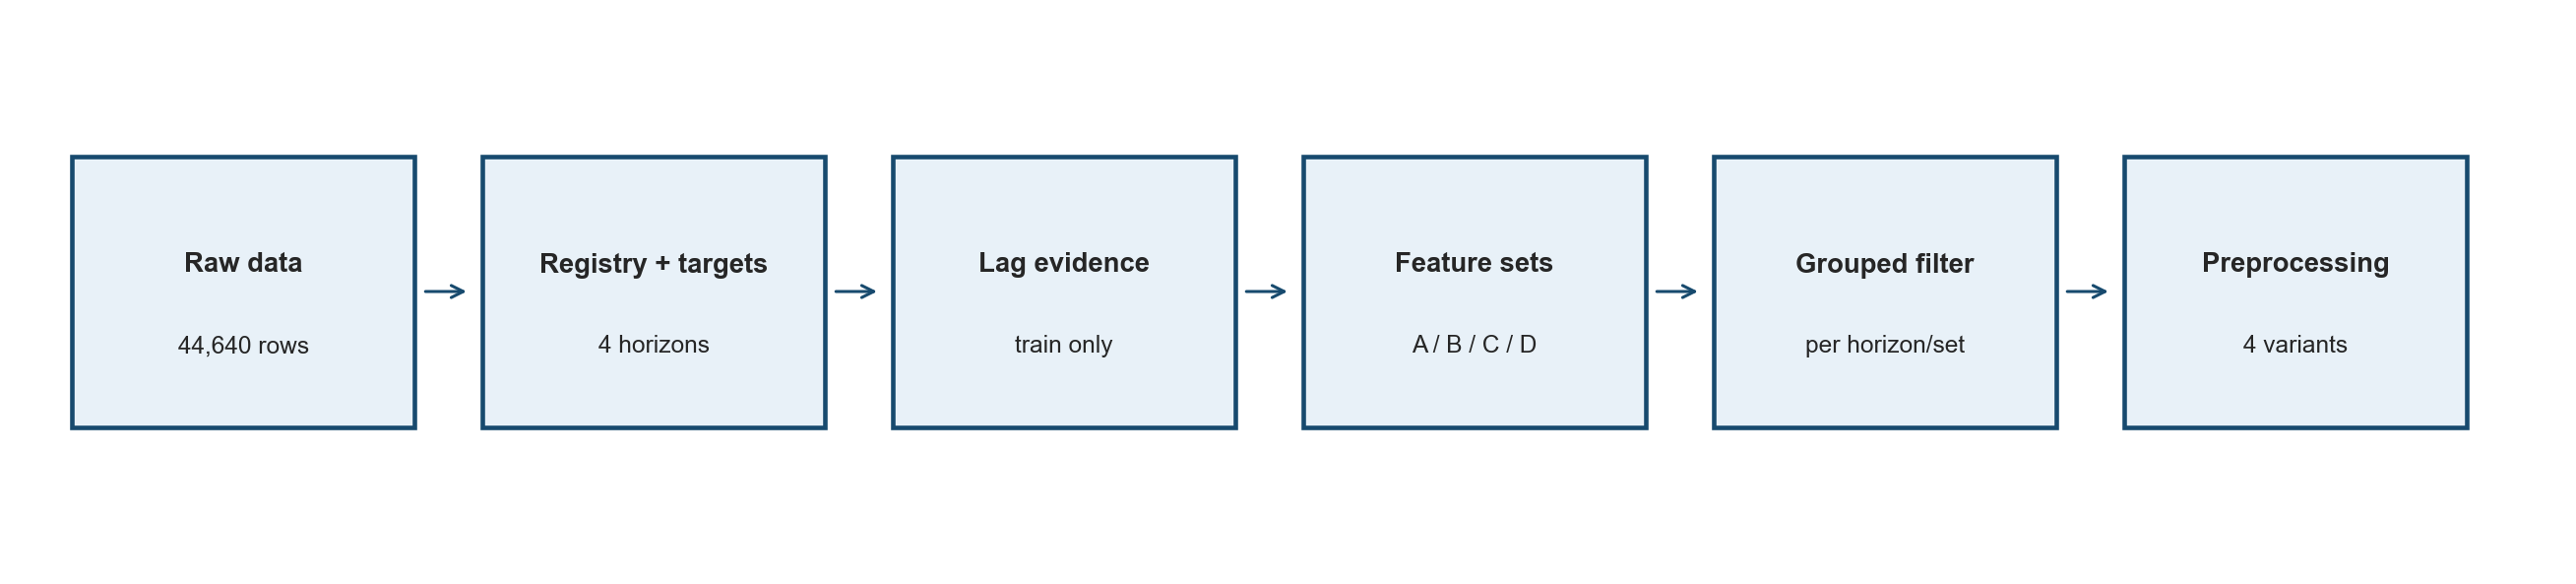
\includegraphics[width=\textwidth]{feature_preparation_artifacts/figures/pipeline_overview.png}\caption{Feature-preparation pipeline: input history, training-only decisions, four hypotheses and leakage-safe prepared splits.}\end{figure}

\section{Notebook 03: direct future-level benchmark}
\subsection{Question, model choices and result}
The first task was $X_{\leq t}\rightarrow\hat y_{t+h}$. For four horizons and four feature sets, all 16 configurations were evaluated with training-target mean, persistence, Ridge, Extra Trees and Histogram Gradient Boosting. Validation selected configurations; test data was used once afterwards.

Ridge used standardised inputs and a compact $\alpha$ search (principally $\{1,10\}$). Trees used matching unscaled, imputed variants. The intent was controlled comparison, not a large unbounded search.
\begin{table}[H]\centering\begin{tabular}{rrrrr}\toprule
\textbf{Horizon} & \textbf{Selected model} & \textbf{MAE} & \textbf{RMSE} & \textbf{vs persistence}\\\midrule
1 min & Set D Ridge & 0.269 & 0.332 & \bad{-67.9\%}\\
5 min & Set D Ridge & 0.275 & 0.338 & \bad{-35.1\%}\\
10 min & Set D Ridge & 0.280 & 0.344 & \bad{-22.6\%}\\
15 min & Set D Ridge & 0.304 & 0.378 & \bad{-27.5\%}\\\bottomrule\end{tabular}\end{table}

The model captured broad operating level but did not beat carrying the latest measured target forward. This negative result was valuable: direct level prediction spends effort reproducing the existing level while persistence is extremely strong at short horizons.

\section{Notebook 04: target-anchored delta forecasting and warnings}
\subsection{Reframing and training design}
The target was changed to movement, not the meaning of the operational output:
\[
\Delta y_{t,h}=y_{t+h}-y_t,\qquad\hat y_{t+h}=y_t+\widehat{\Delta y}_{t,h}.
\]
At prediction time, the model uses present/recent laboratory value and process information, estimates change, then reconstructs future free-acid level. It is valid only if $y_t$ is truly available and fresh.

Inputs were ablated: 21 raw process variables, 178 accepted full exogenous variables, 10 current/past target-history features and a 188-feature hybrid. Ridge and Extra Trees received equal two-candidate tuning budgets. Validation selected hybrid Ridge with $\alpha=10$ at every horizon.
\begin{table}[H]\centering\begin{tabular}{rrrrr}\toprule
\textbf{Horizon} & \textbf{MAE} & \textbf{RMSE} & \textbf{$R^2$} & \textbf{RMSE improvement vs persistence}\\\midrule
1 min & 0.102 & 0.151 & 0.889 & \good{+23.2\%}\\
5 min & 0.113 & 0.169 & 0.862 & \good{+32.3\%}\\
10 min & 0.126 & 0.182 & 0.839 & \good{+34.9\%}\\
15 min & 0.176 & 0.237 & 0.726 & \good{+19.8\%}\\\bottomrule\end{tabular}\end{table}

Accepted engineered features improved raw process input by 10.3--24.2\% depending on horizon. Target history improved full exogenous information by 8.2--12.7\%; full process information improved target history alone by 5.4--23.5\%. Both evidence sources carry complementary predictive association. One minute has lowest absolute error; ten minutes has largest persistence improvement. The operational horizon must also consider needed reaction time.
\begin{figure}[H]\centering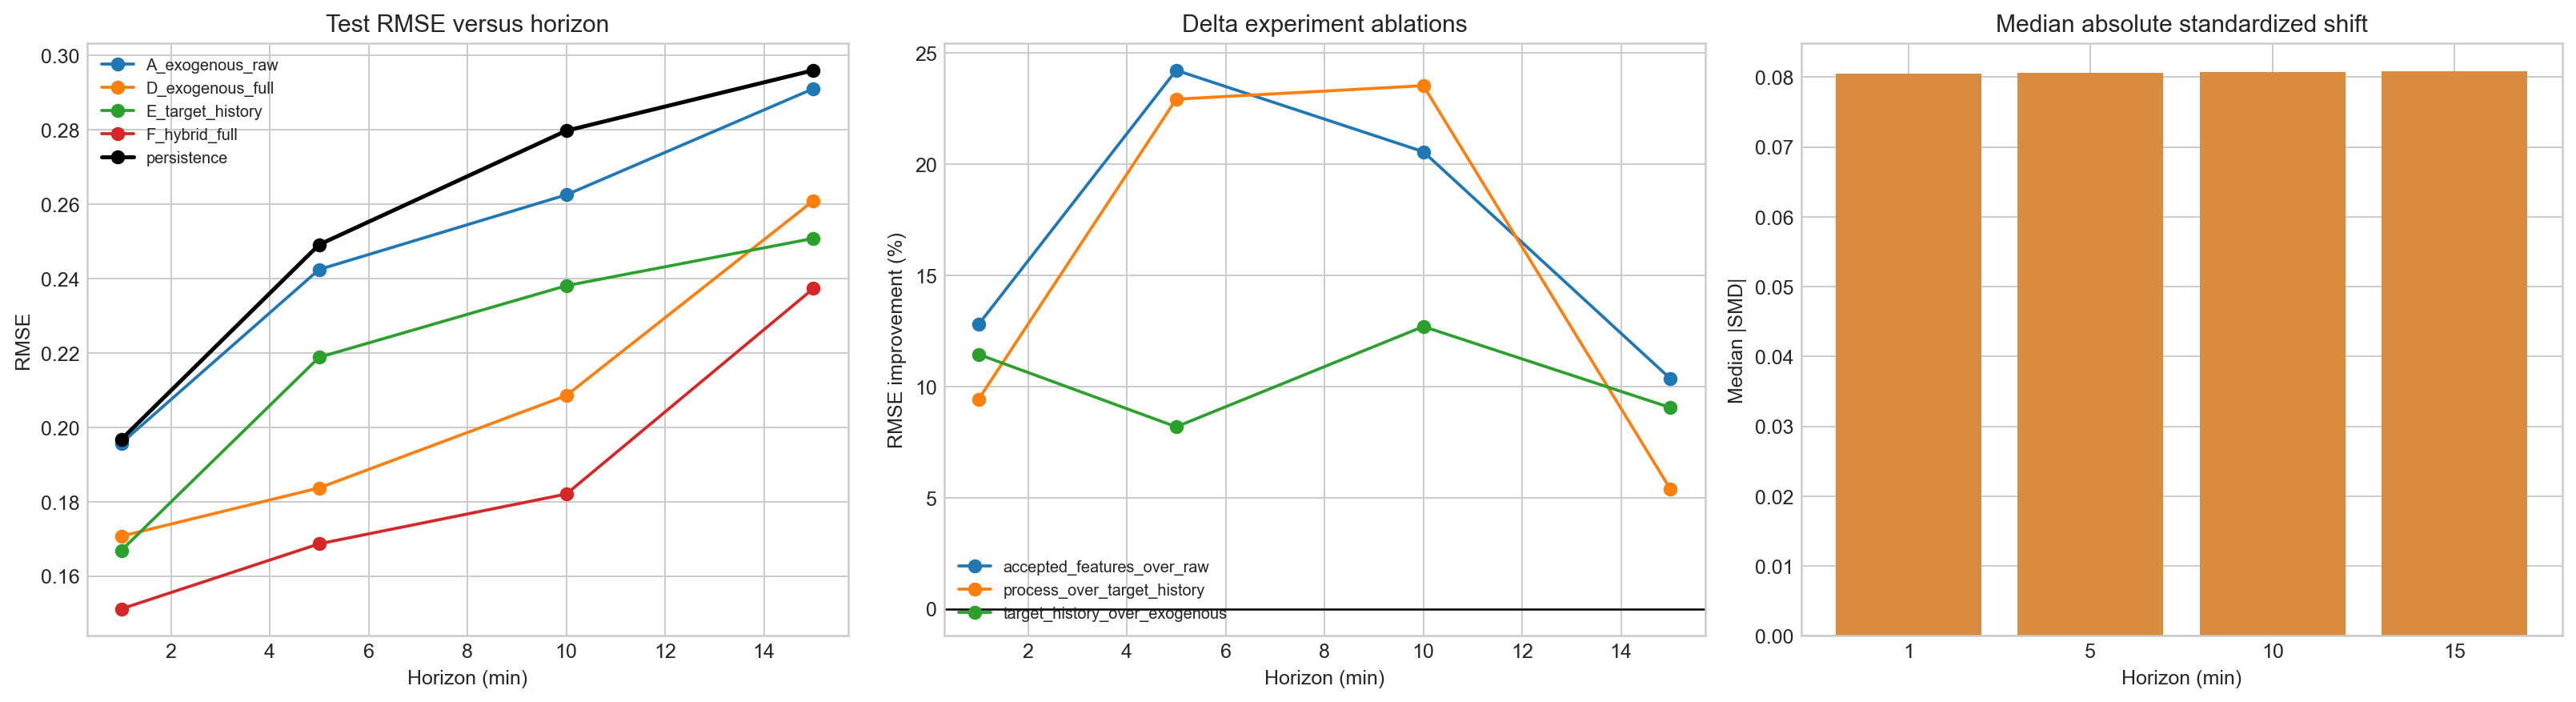
\includegraphics[width=\textwidth]{delta_transition_artifacts/figures/delta_performance_ablation_and_shift.png}\caption{Delta benchmark: performance, feature ablation and distribution-shift diagnostic.}\end{figure}

\subsection{Transition diagnostics}
Candidate transitions were defined by the training 90th percentile of $|\Delta y_{t,h}|$ and extremes by the 95th. A logistic classifier was retained only as a diagnostic. Its precision/recall/F1 at 1, 5, 10 and 15 minutes were 0.141/0.478/0.218, 0.155/0.491/0.235, 0.161/0.512/0.245 and 0.142/0.404/0.210. False-warning rates ranged 0.259--0.288. Fourfold transition weighting slightly helped some transition errors but worsened total RMSE, so it was not retained. No classifier is presented as an operational alarm.

\section{Notebook 05: target-free virtual sensor}
\subsection{Purpose, model choices and result}
The virtual-sensor task is $X_{\leq t}\rightarrow\hat y_t$ without current target, target history or future target columns. It estimates current free acid when only process signals are supplied. Fourteen experiments compared seven model families over raw and full sets: Ridge, PLS, KNN, Extra Trees, HistGradient, XGBoost/LightGBM where available and validation-weighted blends.

Ridge is a transparent regularised linear baseline for correlated signals. PLS is a latent-variable soft-sensor reference. KNN tests similarity to historical operating states. Tree/boosting models test nonlinear thresholds/interactions. Blending is allowed only when validation residuals are complementary.

Validation selected the full-set 50/50 Ridge--LightGBM blend:
\[\hat y_t=0.5\hat y_t^{\mathrm{Ridge,D}}+0.5\hat y_t^{\mathrm{LightGBM,D}}.\]
\begin{table}[H]\centering\begin{tabular}{lrr}\toprule \textbf{Test metric} & \textbf{Training mean} & \textbf{Selected blend}\\\midrule
MAE & 0.355 & \good{0.249}\\ RMSE & 0.454 & \good{0.301}\\ $R^2$ & \textasciitilde0 & \good{0.558}\\ Median absolute error & -- & 0.229\\ 90th / 95th absolute error & -- & 0.459 / 0.536\\\bottomrule\end{tabular}\end{table}

The empirical 90\% interval had 89.7\% January-test coverage with mean width 1.015. It was calibrated from individual Ridge validation residuals while the point estimate is a blend; it is an empirical advisory interval, not a formal guarantee. A training-99th-percentile drift flag marked 1.37\% of test rows, where error was higher.
\begin{figure}[H]\centering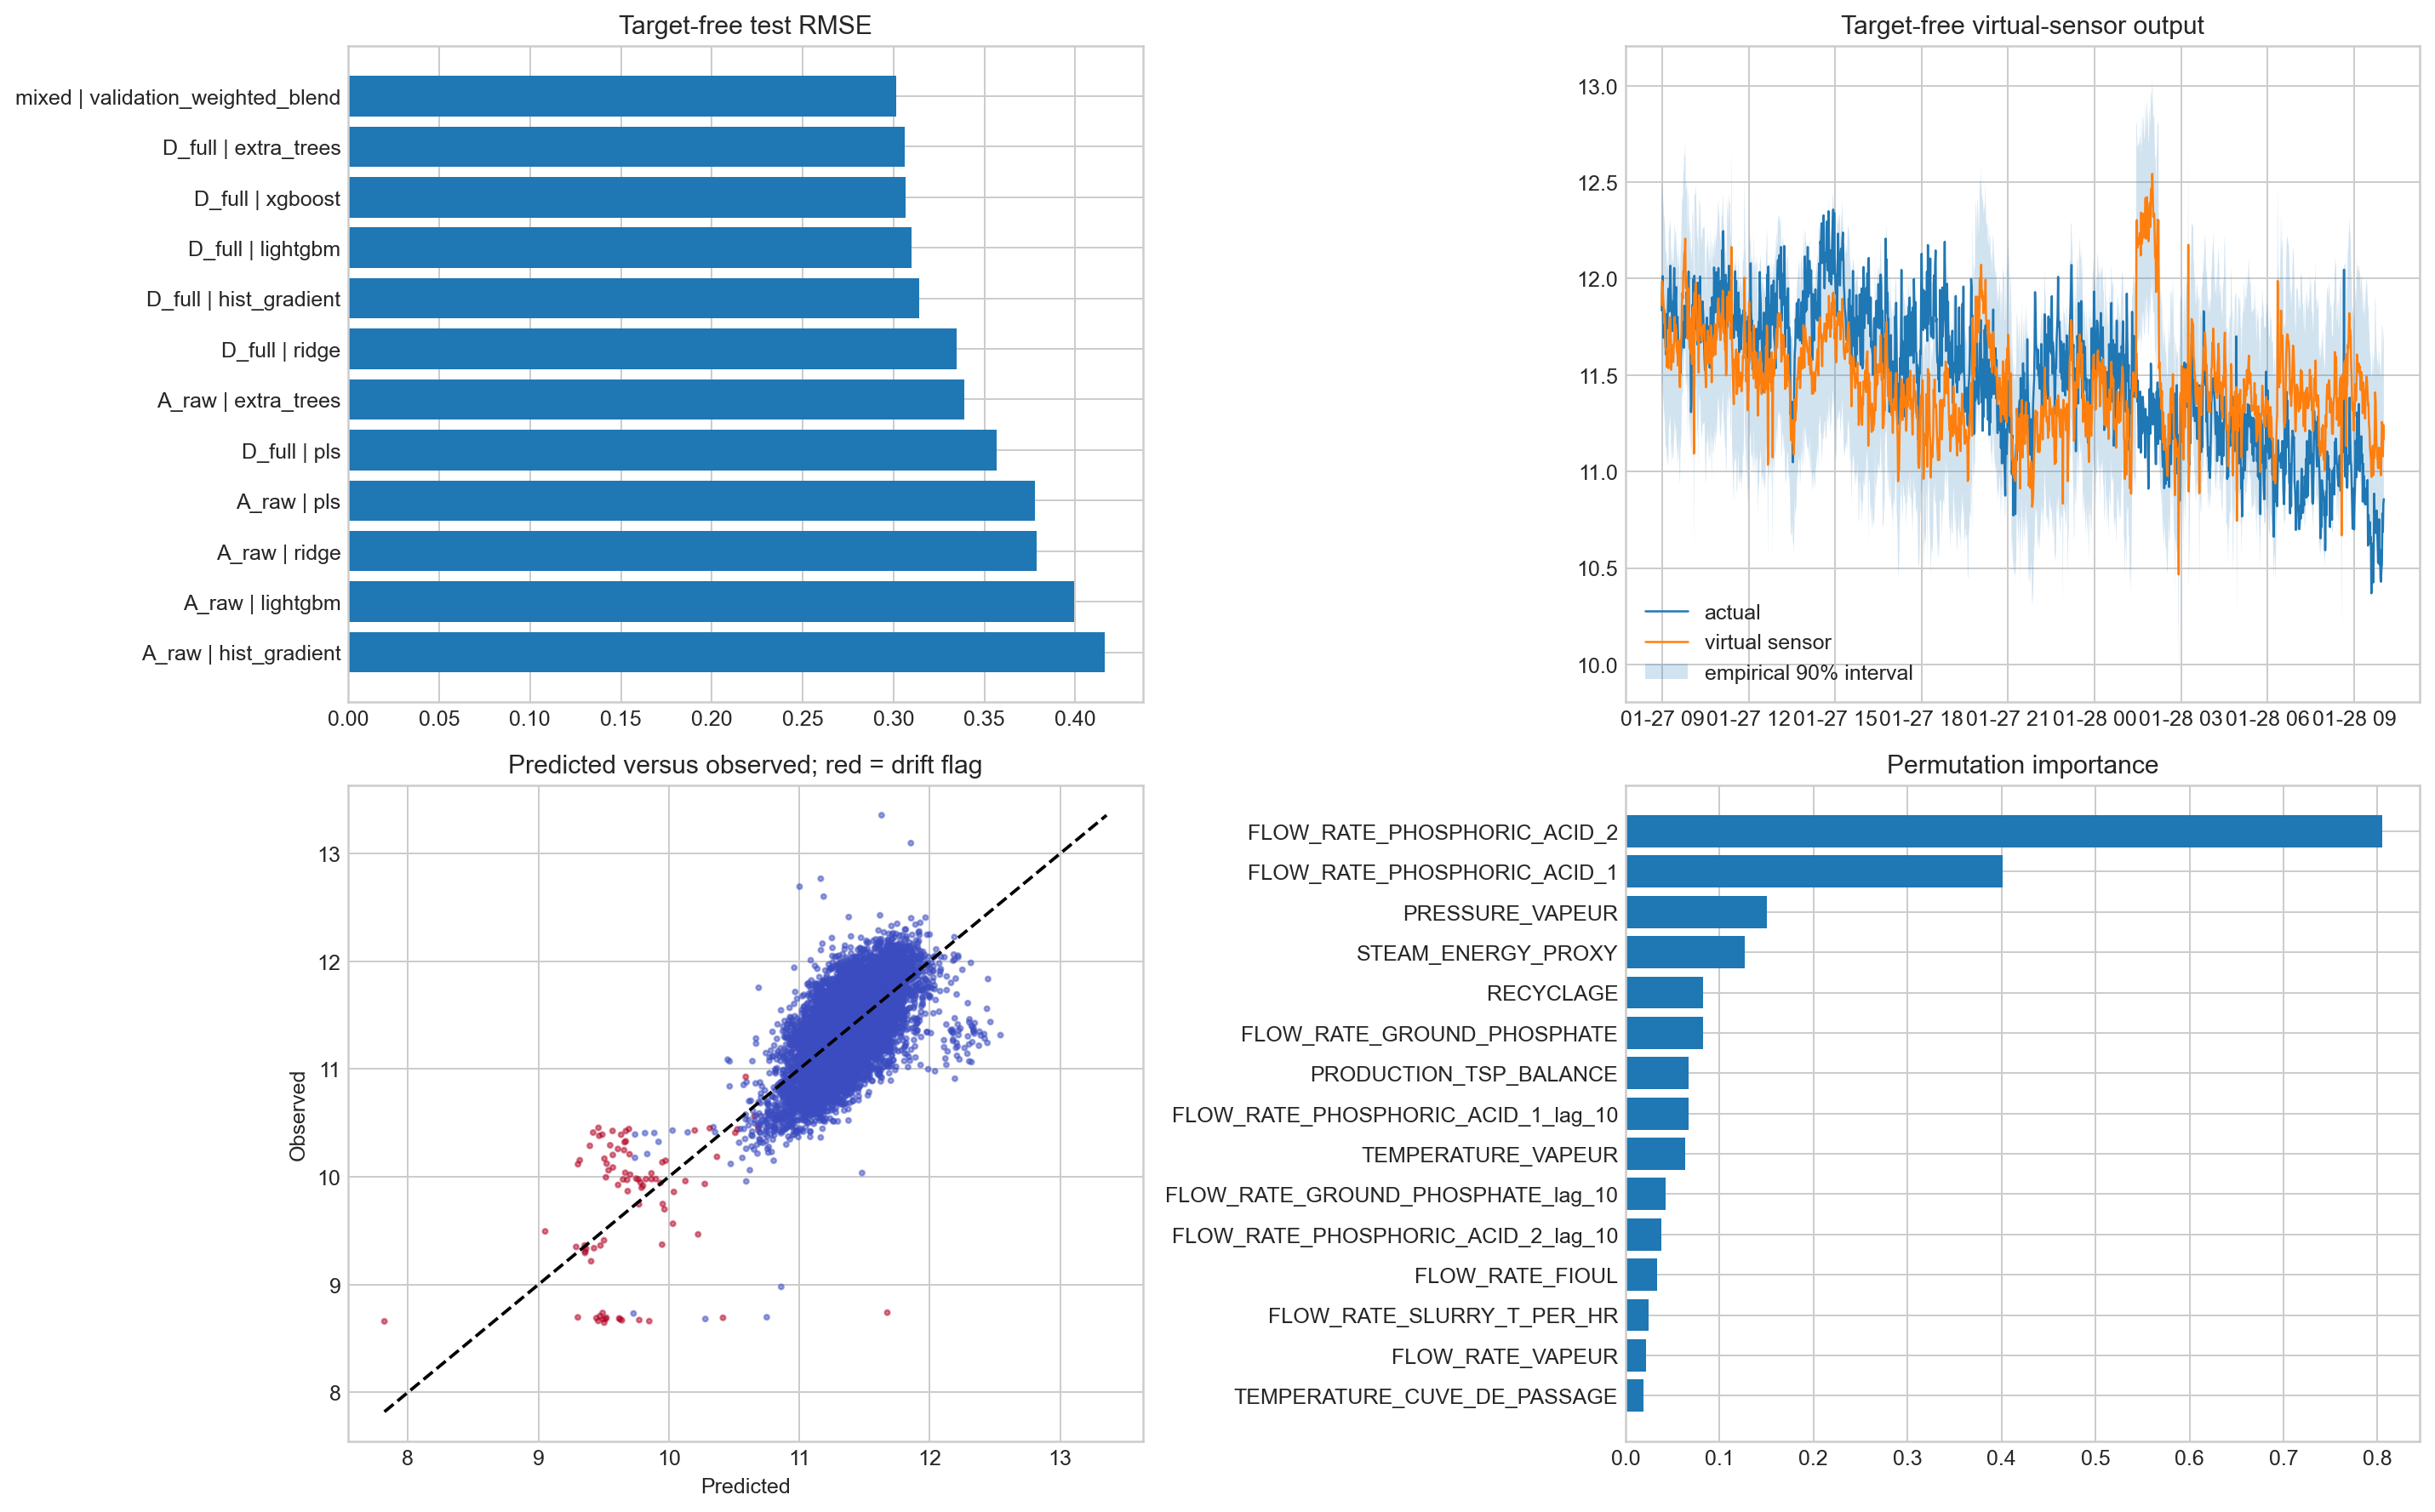
\includegraphics[width=0.86\textwidth]{exogenous_virtual_sensor_artifacts/figures/virtual_sensor_performance.png}\caption{Virtual-sensor comparison and diagnostics. Importance is predictive association, not physical causality.}\end{figure}

\section{Notebooks 06--08: robustness and locality research}
\subsection{Motivation and validation method}
One validation segment is insufficient for dependent one-minute data. Notebook 06 used four expanding chronological blocks, fitting imputation and standardisation inside each fold's preceding training rows. Candidate selection used mean RMSE, RMSE standard deviation and worst-block RMSE; test data was excluded.
\begin{table}[H]\centering\begin{tabular}{lrrr}\toprule \textbf{Candidate} & \textbf{Mean RMSE} & \textbf{RMSE SD} & \textbf{Worst block}\\\midrule
70/30 Ridge--LightGBM & 0.3191 & 0.0762 & 0.4236\\
50/50 Ridge--LightGBM & 0.3201 & 0.0686 & 0.4124\\
Five-cluster Ridge & 0.3280 & \good{0.0396} & \good{0.3522}\\
Global Ridge $\alpha=100$ & 0.3274 & 0.0811 & 0.4353\\
LightGBM (31 leaves) & 0.3483 & 0.0599 & 0.4080\\\bottomrule\end{tabular}\end{table}

The 50/50 blend was average-performance choice. Five-cluster Ridge was more stable in worst-block behaviour. KMeans clusters are data-defined feature-space regions, not validated plant regimes.

Notebook 07 combined the global 50/50 blend with five local Ridge experts. An expert is used only for a sufficiently represented KMeans region, with global Ridge fallback. Fixed local weights and distance gates were tested. The stability-first choice was 80\% local / 20\% global: mean RMSE 0.3217, RMSE SD 0.0412 and worst block 0.3520. It remained within 2\% of the best mean candidate (0.3160 at 40\% local), while lowering worst-block RMSE about 14.7\% versus global-only.

Retrospective January results after refitting are engineering observations, not new selection evidence. Notebook 06 global blend reached MAE 0.2344, RMSE 0.2879, $R^2=0.5970$; Notebook 07 hybrid reached MAE 0.2309, RMSE 0.2889, $R^2=0.5941$. There is no clear overall winner. Notebook 08 retained the discipline that a genuinely later labeled month is required before model replacement.

\section{Analytics and dashboard work}
The interactive analysis dashboard supports default data or CSV upload, trajectory plots with axes, missingness, pairwise correlation/scatter analysis, data observations, candidate-transition windows and model outputs. Transition views show when a window occurred, consecutive duration, strongest sensor drivers, later target response when labels exist and prediction error when a compatible prediction run exists.

The native Windows advisory dashboard reads only runtime output. It has a dark industrial theme, current prediction/status/input-quality cards, trend chart, selectable 60/360/720-point history, hover crosshair and nearest-point tooltip, imputed-input markers, delta versus previous prediction and a heartbeat watchdog. It uses read-only SQLite WAL access and deterministic closing; it never writes audit data.

The green process-change line in transition displays is multivariate normalised sensor movement. It is not target change, causal attribution, confirmed event type or a model prediction.

\section{Industrial deployment architecture}
\subsection{Macro architecture and safety boundary}
\begin{center}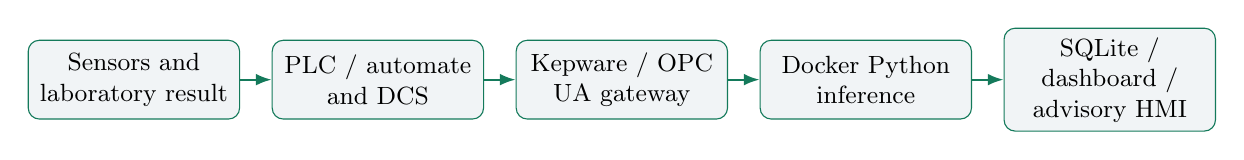
\begin{tikzpicture}[node distance=4mm and 4mm,box/.style={draw=Green,rounded corners,fill=Light,minimum height=10mm,text width=2.45cm,align=center,font=\small},arr/.style={-{Latex[length=2mm]},thick,draw=Green}]
\node[box](s){Sensors and laboratory result};\node[box,right=of s](p){PLC / automate and DCS};\node[box,right=of p](k){Kepware / OPC UA gateway};\node[box,right=of k](d){Docker Python inference};\node[box,right=of d](h){SQLite / dashboard / advisory HMI};
\draw[arr](s)--(p);\draw[arr](p)--(k);\draw[arr](k)--(d);\draw[arr](d)--(h);\end{tikzpicture}\end{center}

Sensors measure process variables; actuators (valves, pumps, motors) change the plant. PLCs execute fast deterministic local logic; the DCS coordinates wider control, HMI and supervision. The ML service is neither. It never writes setpoints, commands, interlocks or safety logic. Its failure must leave the plant safe.

Kepware is a translation gateway: southbound it uses approved vendor/protocol drivers to reach controllers; northbound it exposes configured tags through OPC UA. A real deployment needs a Windows Kepware host, endpoint/security certificates, network/firewall route and validated Node IDs. Node IDs are externalised in configuration, never hard-coded in Python.

\subsection{Stage 1 CSV-replay laboratory implementation}
\begin{enumerate}
\item A simulator container replays historical CSV rows as OPC UA process tags, source timestamp and sequence/commit tag.
\item The inference container subscribes to the sequence tag rather than repeatedly polling each tag.
\item It reads sequence before and after values; a snapshot is accepted only when both agree, avoiding a mixed two-row snapshot.
\item A quality shield checks OPC quality, chronology, impossible values, excessive simultaneous missingness and timestamp gaps. Ordinary isolated missing cells may be imputed by the trained pipeline and are marked \code{IMPUTED}.
\item Accepted snapshots enter a chronological buffer, then feature generation, saved preprocessing and model inference.
\item Predictions/audit records go to \code{runtime/predictions.sqlite3} in WAL mode; health goes to \code{runtime/health.json}.\end{enumerate}

The target-free service uses the five-cluster Ridge virtual sensor as stability-oriented candidate. Target-anchored operation remains distinct because it needs explicitly fresh manual laboratory result.

\subsection{Warm-up, reliability, Docker and database}
The maximum feature lookback is 30 minutes, so $30+1=31$ rows are needed after cold start. The preferred production improvement is historian backfill, followed by carefully validated persistent-buffer restoration. The laboratory simulator has acknowledgement flow control so it cannot outrun inference; it is laboratory-only and must remain disabled with real Kepware/plant sources.

The service detects connection closure/sequence reset, creates fresh run ID on reconnect, clears incompatible history, reports \code{DISCONNECTED}, then reconnects. The dashboard heartbeat watchdog (30/90/180 seconds or off) detects frozen health updates but does not control equipment.
\begin{table}[H]\centering\begin{tabularx}{\textwidth}{L{0.24\textwidth}Y}\toprule \textbf{Status} & \textbf{Meaning}\\\midrule
STARTING / CONNECTED & Service begins or has OPC session but insufficient history.\\
WARMING\_UP & Valid history is collected; at least 31 rows are required.\\
RUNNING & A recent accepted snapshot has produced model-ready state.\\
DATA\_ERROR & Serious quality/chronology/coverage condition, not ordinary isolated imputation.\\
DISCONNECTED & OPC connection failure/reset detected; automatic reconnect attempted.\\\bottomrule\end{tabularx}\end{table}

Docker Compose runs simulator and inference on an isolated network. The native Windows PySide6/PyQtGraph dashboard is compiled with PyInstaller and launched by a batch launcher that starts containers, opens dashboard, then stops containers when it closes. SQLite WAL provides local single-host audit data with concurrent read-only dashboard access. Production still needs retention, backup, access-control and historian decisions.

\section{Verification completed}
The CSV-replay laboratory path was executed end-to-end: images built, OPC UA server started, inference connected/subscribed, saved artifacts loaded, health/SQLite output generated and dashboard reads tested. Engineering failures were investigated: Docker Hub timeouts, PowerShell argument forwarding, missing OpenMP runtime for LightGBM, replay faster than processing, duplicate timestamps, missing initial prediction file and unreadable OPC logs.

Latest reliability tests included sustained replay and controlled simulator restart. A healthy observed state reached \code{RUNNING}, 180 buffered rows, zero buffer resets and heartbeat activity. Stopping the simulator gave \code{DISCONNECTED}; restarting created a new run, warmed up and returned to \code{RUNNING}. Seventeen automated deployment/dashboard tests passed after resilience/UI changes. These validate software behaviour, not plant process validity.

\section{Limits, risks and validation requirements}
\begin{table}[H]\centering\begin{tabularx}{\textwidth}{L{0.30\textwidth}Y}\toprule \textbf{Limitation or risk} & \textbf{Required treatment}\\\midrule
One month only & Freeze candidates; evaluate a later labeled month without retuning; then use rolling-origin multi-month validation.\\
Manual laboratory target & Define timestamp, freshness, sampling/analysis delay and reconciliation policy before target-anchored operation.\\
Uncertain units/streams & Confirm units/material basis for acid, phosphate, fuel, steam, wash liquid and recyclage; verify slurry t/h versus combined $m^3/h$.\\
Statistical regimes & Match against operator logs: startup, shutdown, maintenance, cleaning, grade and disturbances.\\
Feature importance & Predictive association only; never claim causality or propose changing unconfirmed controllable variables.\\
Intervals/drift & Recalibrate on independent multi-month residuals; current output is advisory diagnostic.\\
OPC/DCS integration & Obtain endpoint, certificates, security policy, Node IDs, quality semantics, firewall route and IT/OT approval.\\
Operational use & Begin in read-only shadow mode; compare live outputs to lab results; no automatic control.\\\bottomrule\end{tabularx}\end{table}

\section{Recommended next milestones}
\begin{enumerate}
\item Obtain a later month of timestamped process data and lab \code{SLURRY_FREE_ACID}; freeze candidates and run external evaluation without retuning.
\item Agree operational contract: current-time virtual sensing, target-anchored warning or both, with lab freshness and error/warning cost.
\item Validate proxy assumptions, controllability and candidate transitions with process engineers and operating records.
\item Add historian backfill/persistent recovery, retention and audit policies before sustained shadow operation.
\item Connect to secured laboratory Kepware, validate tags/certificates/reconnect, then run production read-only shadow mode.
\item Select an operational model only after multi-month evidence. Deep sequence models are not the immediate priority.\end{enumerate}

\section*{Conclusion}\addcontentsline{toc}{section}{Conclusion}
The work progressed from exploration to leakage-controlled forecasting, a target-free soft sensor, dashboards and reproducible advisory deployment. The strongest result is target-anchored delta forecasting beating persistence at all tested horizons in January. The equally important caution is that the target is manual, feature semantics are partly provisional and data covers one month. External validation and read-only industrial shadow mode are the correct next steps, not autonomous control.
\end{document}
